
%===============================================================================================================%
\section{Residuals and Diagnostics}
\begin{itemize}
\item For a given value X of the independent variable, the value predicted by regression line $\hat{y}$ is often called the \textbf{fitted
	value} of the dependent variable. 
\item The difference between the observed value Y and the fitted value Y
is called the residual for that observation and is denoted by \textbf{e}:
\[e= Y-\hat{Y}\]

\item (Important for later: Residuals represent unexplained (or residual) variation after fitting a regression
model. )
For the example used in this class, the residuals are very small.
\end{itemize}



A residual plot is obtained by plotting the residuals e with respect to the independent variable X or,
alternatively with respect to the fitted regression line values $\hat{Y}$. Such a plot can be used to
investigate whether the assumptions concerning the residuals appear to be satisfied.

\subsection{Asummption of Constant Variance}
\begin{itemize}
\item Homoscedascity (also known as constant variance) is one of the assumptions required in a
regression analysis in order to make valid statistical inferences about population relationships.

\item Homoscedasticity requires that the variance of the residuals are constant for all fitted values,
indicated by a uniform scatter or dispersion of data points about the trend line (i.e. "The Zero Line").
\item From the above plot, we can conclude that the constant variance assumption is valid. We can also
see that the mean value of the residuals is close to zero. \textit{(Theoretically it is precisely zero)}.
\end{itemize}

\begin{figure}
\centering
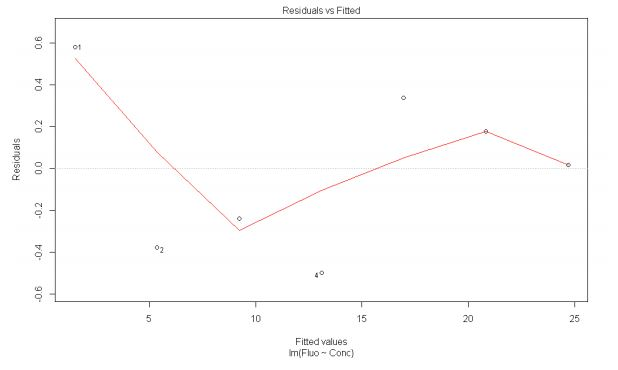
\includegraphics[width=1.1\linewidth]{ResidPlot1}
\end{figure}

\subsection{Normality of Residuals}
Additionally, the linear model approach requires this assumption that the residuals are normally
distributed. We can use a Q-Q plot to assess the normality of residuals.
\begin{figure}
\centering
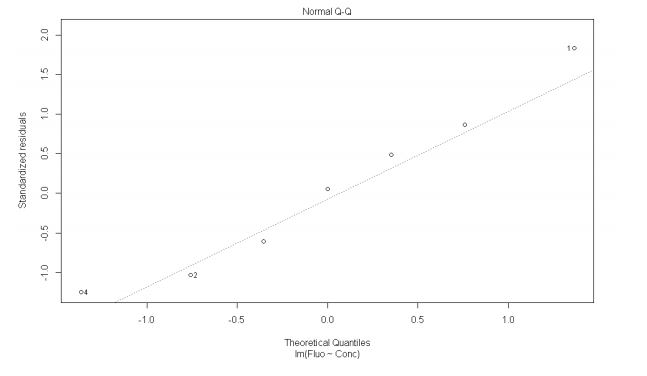
\includegraphics[width=1.1\linewidth]{ResidPlot2}
\end{figure}

\newpage
\section{Regression Diagnostics}

An excellent review of regression diagnostics is provided in John Fox's aptly named \textbf{Overview of Regression Diagnostics}. Dr. Fox's car package provides advanced utilities for regression modeling.
\begin{framed}
	\begin{verbatim}
# Assume that we are fitting a multiple linear regression
# on the MTCARS data
library(car)
fit <- lm(mpg~disp+hp+wt+drat, data=mtcars)
	\end{verbatim}
\end{framed}

This example is for exposition only. 
We will ignore the fact that this may not be a great way of modeling the this particular set of data!

\subsection{Bivariate Outliers}

\begin{framed}
	\begin{verbatim}
	# Assessing Outliers
	outlierTest(fit) # Bonferonni p-value for most extreme obs

	\end{verbatim}
\end{framed}
\begin{framed}
	\begin{verbatim}
qqPlot(fit, main="QQ Plot") #qq plot for studentized resid 
leveragePlots(fit) # leverage plots
	\end{verbatim}
\end{framed}
leverage plot click to view

\subsection{Influential Observations}


av plots Cook's D plot influence plot click to view
%=========================================================== %
\subsection{Non-normality}
\begin{framed}
\begin{verbatim}
# Normality of Residuals
# qq plot for studentized resid
qqPlot(fit, main="QQ Plot")

# distribution of studentized residuals
library(MASS)
sresid <- studres(fit) 
hist(sresid, freq=FALSE, 
main="Distribution of Studentized Residuals")
xfit<-seq(min(sresid),max(sresid),length=40) 
yfit<-dnorm(xfit) 
lines(xfit, yfit)
\end{verbatim}
\end{framed}
qq plot histogram of studentized residuals click to view
%============================================================== %

%============================================================== %
Multi-collinearity
\begin{framed}
\begin{verbatim}
# Evaluate Collinearity
vif(fit) # variance inflation factors 
sqrt(vif(fit)) > 2 # problem?
\end{verbatim}
\end{framed}
%============================================================ %
\subsection{Nonlinearity}
\begin{framed}
	\begin{verbatim}
# Evaluate Nonlinearity
# component + residual plot 
crPlots(fit)
# Ceres plots 
ceresPlots(fit)
\end{verbatim}
\end{framed}
component plus residual plot Ceres plots click to view


# Assessing Outliers
outlierTest(FitAll) # Bonferonni p-value for most extreme obs
qqPlot(FitAll, main="QQ Plot") #qq plot for studentized resid 
leveragePlots(FitAll) # leverage plots
leverage plot click to view



av plots Cook's D plot influence plot click to view
Non-normality
# Normality of Residuals
# qq plot for studentized resid
qqPlot(FitAll, main="QQ Plot")
# distribution of studentized residuals
library(MASS)
sresid <- studres(FitAll) 
hist(sresid, freq=FALSE, 
main="Distribution of Studentized Residuals")
xFitAll<-seq(min(sresid),max(sresid),length=40) 
yFitAll<-dnorm(xFitAll) 
lines(xFitAll, yFitAll)
qq plot histogram of studentized residuals click to view



crPlots(FitAll)
# Ceres plots 
ceresPlots(FitAll)
component plus residual plot Ceres plots click to view
Non-independence of Errors
